\chapter{Interpretação Abstrata} \label{fundamentacao_ia}

O conceito de \gls{IA} foi introduzido por \citeonline{cousot_abstract_1977}, e 
sumarizado em \citeonline{cousot_abstract_2008}. Outros autores, como 
\citeonline{mine_weakly_2004} e \citeonline{bygde_abstract_2006}, também 
descrevem a \gls{IA} e os \glspl{dominioAbstrato}, talvez até de forma clara e 
simples.

Softwares são construídos para atender a alguma finalidade. Quando deseja-se 
verificar se este software atende a esta finalidade, é preciso formalizar o seu 
funcionamento, seja através de mecanismos de linguagem, ou externamente ao 
código-fonte original. À este formalismo, damos o nome de \emph{especificação}. 
É com base nestes requisitos que ocorre a verificação; ou seja, que pode-se 
afirmar, com certo nível de confiança, que a \emph{semântica} (o que o software 
faz, de fato) equivale ou se aproxima do que é esperado.

Em resumo, a \gls{IA} tem como objetivo:

\begin{itemize}
    \item Prover uma teoria sólida e coerente para auxiliar no entendimento e 
    construção de ideias, conceitos e conclusões acerca dos processos de 
    análise e verificação formal de softwares e programas computacionais.
    
    \item Auxiliar no design de ferramentas, utilitários e infraestrutura de 
    análise e verificação formal de programas.
\end{itemize}

A \gls{IA} é baseada nos conceitos de \glspl{reticulado} e 
\glspl{conjuntoOrdenado}. 

    \section{Conjuntos e Reticulados}

    \TODO{Apesar de já ter uma entrada no glossário para os dois termos, seria 
    melhor explicar o que é reticulado aqui, pois o tema é importante para as 
    proposições que se seguem.}

    \section{IA e Domínios Abstratos}
    
    A \gls{IA} é uma teoria de abstração, onde tenta-se \emph{aproximar} um 
    \emph{estado abstrato} (esperado, a semântica do programa derivada da 
    análise) de um \emph{estado concreto} (real, descrito por uma especificação 
    ou testado em tempo de execução). Este processo de aproximação no geral 
    propriedades do software que são interessantes ou relevantes à verificação, 
    e ignora todos os outros.
    
    \TODO{Falar sobre solidez e completude.}
    
        \subsection{Domínios não-relacionais}
        \subsection{Domínios Relacionais}
        
        
    \section{Domínio dos Octógonos}
        \subsection{Vantagens e Diferenciais}
        \subsection{Matrizes de Diferenças}
        \subsection{Operadores}


\chapter{Computação Paralela} \label{fundamentacao_cl}
    \section{Conceitos gerais}
    \section{OpenCL}
        \subsection{Arquitetura Geral}
        \begin{figure}[t]
            \centering
            \caption{Modelo de memória do OpenCL.}
            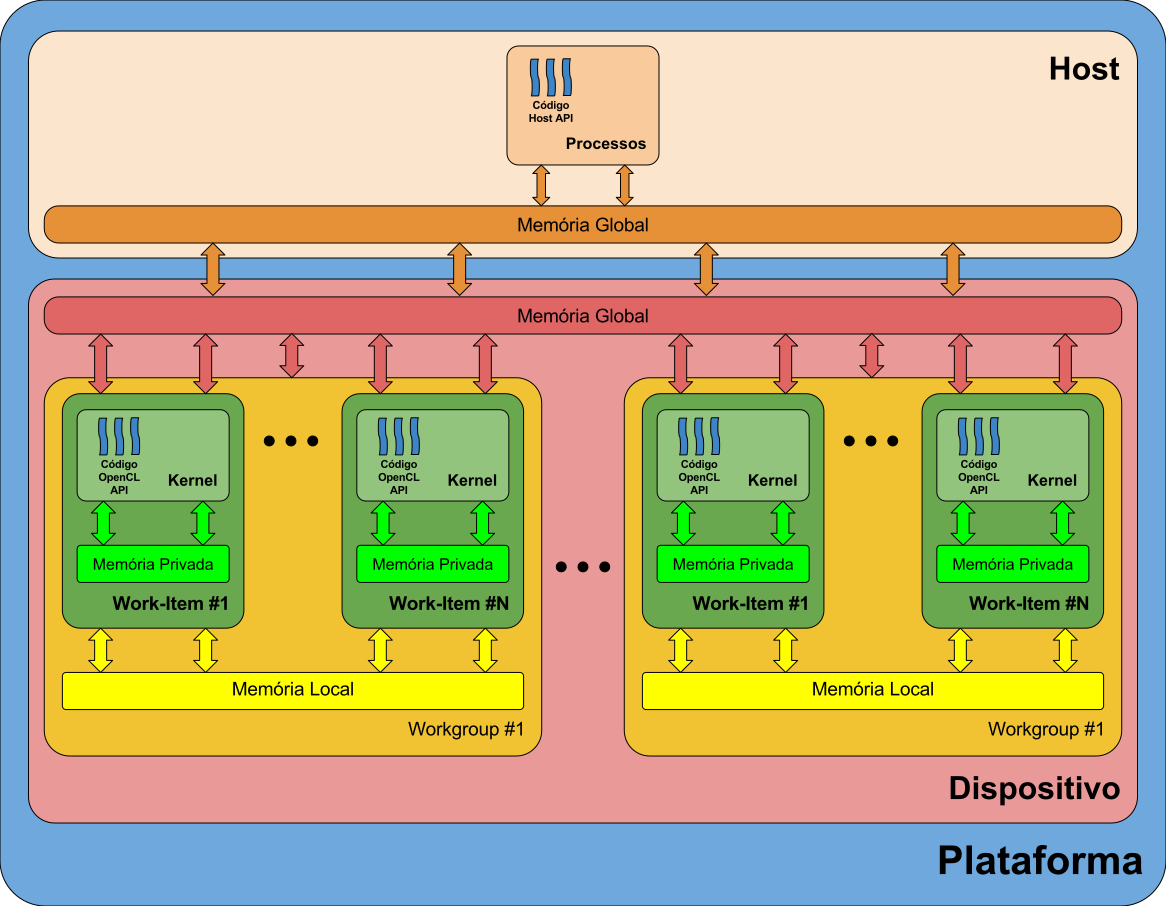
\includegraphics[width=\textwidth]{opencl-modelo-memoria}
        \end{figure}
        \subsection{Workgroups, Work-items e Memória}
        \subsection{Exemplos}
        